\chapter{Introduction}
\label{the-introduction}
% This should cover the problem the thesis addresses, the aims and questions, the thesis structure, a summary of the main findings and a discussion on the thesis' contribution. It should prime the reader for what's about to come by providing an overview of what lies ahead.

% Establish your research territory by situating your research in a broader context. 
% Establish and justify your niche by describing why your research is needed. 
% Explain the significance of your research by describing how you conducted your research.
Billions of people use mobile apps on two main mobile platforms, Google Android and Apple iOS, and their related operating systems.  Android is integrated into additional mobile platforms including Kindle OS and various Original Equipment Manufacturers (OEM), particularly Huawei with HarmonyOS. There are millions of these mobile apps developed by millions of developers across the globe. Failures in these apps can adversely affect the experiences of end-users, businesses who provide apps, and/or goods and services provided through mobile apps. 

%\subsection{The essence of analytics}
Software is not perfect; it is formed through numerous human endeavours using flawed tools and techniques. 
Bugs are ubiquitous in software, and no practical software is bug-free. Even one of the most respected software engineers, Donald E. Knuth, recognises, publicly acknowledges, \emph{and pays for}, bugs found in his creations~\citep{knuth_trutex, wikipedia__knuth_reward_checks_2020}. \emph{``You are entitled to a reward of at least 0x$1.00 \nobreak\hspace{.16667em plus .08333em} ($2.56) if you are the first person to report a bona-fide error not on those lists."}~\citep{knuth_the_bank_of_san_serriffe}. And self-aware developers expect that there will be bugs in their software. Nonetheless those involved can improve software through their choices and practices.

Analytics exist and are used across and throughout software development practices, and they can be used to better understand and improve these practices and the resultant software~\citep{buse_analytics_2010, buse2012_information_needs_for_software_development_analytics, menzies2018_unreasonable_effectiveness_of_software_analytics}.

Broadly, this research aims to understand whether mobile analytics can help developers to improve the reliability of their apps. A second applied research area emerged as various flaws and limitations were discovered in the various mobile analytics services, to discover and categorise the flaws and limitations, and to consider some of the effects on actually improving app quality given these flaws and limitations. 

This research focuses on the most used operating system -- Android -- in it's most popular and mature platform -- Google Android -- to discover whether mobile analytics can help developers improve the stability of their apps by fixing bugs that adversely affect their stability. A default mobile analytics service, called Android Vitals~\footnote{Android Vitals is integrated into Google Play Console which provides additional functionality including app store metrics, ratings and reviews, release management, and so on.}, is integrated into the Google Android platform and available free of charge for all developers of apps in the Google Play App store. So, it was selected as the core analytics tool for this research, as it is prevalent, and also one of the quality signals Google uses to decide whether to promote apps in its app store. This default mobile analytics service is complemented with research in additional analytics tools that include in-app crash reporting (how they do so is discussed in \href{{app:crash-recording-and-reporting-in-android}}{\nameref{app:crash-recording-and-reporting-in-android}}) to provide perspective and contrast on their various characteristics and capabilities. In app crash reporting is used in at least 80\% of Android apps in Google play according to AppBrain's analysis of Crash Reporting libraries~\footnote{\url{https://www.appbrain.com/stats/libraries/tag/crash-reporting/android-crash-reporting-libraries}}.


In-app crash reporting is not a panacea. Not all apps use it for various reasons, not all crashes are reported by in-app crash reporting; for instance crashes that occur when the app starts, or while an app is still being initialised, may not be detected or reported. And not all failures are crashes, for instance Google Android and Huawei AppGallery consider application freezes, known as ANRs, to be failures too. Therefore this research takes a holistic approach to managing failures that extends beyond the analysis of crashes reported using in-app crash reporting.   % SHOULD-DO forward-reference to a discussion on crashes at startup and comments made by the Google Play Console PM about these types of crashes.

Stability is a prerequisite for an app to be viable in the marketplace, and several key app stores clearly state unreliable apps (~\emph{e.g.} apps that crash) will be marked down and possibly ejected from the app store~\citep{appleappstore2021_app_completeness, google_play_policy_center_broken_functionality, huaweidevelopers_appgallery_review_guidelines}. For example, Apple states~\emph{``On average, over 40\% of app rejections are for Guideline 2.1 – Performance: App Completeness."}~\citep{appleappstore2021_review_avoiding_common_app_rejections} with crashes and debugs listed as the first rejection reason. % Crashes are undesirable yet commonplace; therefore one of the key software qualities in use where analytics may be able to help measure and improve reliability for end users. 
Crashes are undesirable yet commonplace; therefore they are a good candidate for evaluating how analytics may be able to a) help measure them and b) help developers to address them, in order to improve the reliability of mobile apps for end users.

% See also a developer's question about releasing iOS apps with known crashes https://developer.apple.com/forums/thread/68770

Even leading technology companies release software that crashes some have the misfortune to release software that crashes many other apps inadvertently, as Google discovered in Spring 2021~\citep{bbcnews2021_google_fixes_crashing_android_app_issues}. App developers, including the BBC for their iPlayer app, posted advice to end users about the issue in Google Play~\citep{bbc_iplayer_app_april_2021_webview_information} as the adverse effects of the bugs introduced by Google were so widespread.

\medskip
\textbf{Surviving as an app developer}: Software app developers need to deliver software that can be used successfully by end users. To do so they need to be able to create software, package it as an app, and distribute it so it is available to end users. 
%
They need to do so in a timely manner - perfection may be too long to wait for! Therefore developers need to balance and make tradeoffs in the work they do and don't do. \emph{``Bad decisions cost money (and reputation) so we need better tools for making better decisions."}~\citep[p.115]{tantithamthavorn2021_actionable_analytics_tell_me_what_to_do}. The article also observes developers also need to decide what to avoid doing. Therefore developers need help to decide which failures are appropriate to fix now (and which to leave be).

End users need to be able to install and use the app. If the app is sufficiently usable and useful and behaves adequately, they may continue to use it. Developers cannot assess \emph{a priori} whether their app will meet the needs and expectations of users, or the needs of their stakeholders. 
% Briefly explain why they can't...
%  - Product/Market fit
%  - Marketability of apps~\citep{nayebi2017version}, via App Store Effects paper: ``Nayebi et al. subsequently investigated open-source app versions that are not shipped into the app store [46], introducing the concept of release ‘marketability’. To this end, they surveyed 22 developers, the majority of which (95 percent) state that market acceptability of a mobile app release is more important than that of traditional software."
%  - Competition in the app store
%  - They're not in control of their destiny, the app store and the customers decisions have a major impact
%  - Adopting of the app and use of the app 
% - Survivorship in the app store ecosystems and what devs can do to increase their app's survival~\citep{lee2014_determinants_of_mobile_app_success_evidence_from_the_app_store_market} Seller [app developer]-level decisions, app-level decisions, user response to the decisions. It doesn't discuss app store algorithms or their effects. c.f. the more recent articles on iTunes rankings of apps from Medium.com 
In short, they cannot predict whether their app will thrive.


\medskip
\textbf{Crashes can leave indelible, adverse, results}. An increase in crashes led to an increase in `churn'~\footnote{Churn is also known as attrition and is used to measure users who leave a collective group over a specific period~\url{https://en.wikipedia.org/wiki/Churn_rate}.} of up to six times the average rate of churn according to an industry report ~\citep{levy2016_crash_and_churn_report, levy2017_the_crash_and_burn_report_findings}~\footnote{Note: Apteligent was acquired by VMWare in 2017 and few of their online materials remain available.}. % A counter point is that a few organisations can survive crashes in their app, for instance Facebook according to https://9to5google.com/2016/01/04/facebook-intentionally-made-its-android-app-crash-to-test-how-addicted-users-are/ However this is not likely to be the norm for other app developers who lack the scale and pull of Facebook's platform.
In terms of bugs mobile developers face,~\emph{``... automatic in-app crash reporting is the most prolific channel of reporting bugs..."}~\citep{alsubaihin2019app_store_effects_on_software_engineering} % Full sentence: While automatic in-app crash reporting is the most prolific channel of reporting bugs, the one mostly prioritised by our respondents is user reviews in app stores.
-- presumably as there are many crashes in mobile apps, otherwise it wouldn't be a prolific source. Therefore, one success factor for developers of mobile apps is in addressing crashes so they stop being a prolific source of bugs. 

A survey in Germany reported that the most important annoyance for users was instability, ~\emph{i.e. ``instability (app crashes at startup or in certain cases) with 41\% of all responses"}~\citep{nitze2015_a_survey_on_mobile_users_sq_perceptions_and_expectations}.  %Then, users were asked (unsupported) for what they find annoying about using mobile apps. The most important aspect mentioned was instability (app crashes at startup or in certain cases) with 41% of all responses
%SHOULD-DO extend this paragraph with other references. For now I've merged it with the next paragraph.
%
Conversely, Android apps that score highly in terms of stability may be selected to be promoted and featured in Google Play. One of the developer-oriented Google Play Guides provides an imperative: `Improve your app’s quality and discoverability'~\citep{android_store_listing_guide} which combines with the Google Play Guide on Android Vitals. This states: ~\emph{``Apps whose metrics are higher have greater promotability, which raises their ranking in Google Play Store searches. They also are more likely to be eligible for the New \& Updated and Editor's Choice collections on Google Play, and to be nominated in the Google Play Awards."}~\citep{android_android_vitals_guide}. % See also https://blog.embrace.io/top-5-reasons-your-app-is-losing-discoverability-on-google-play-store/


% \yijun{Should talk about quality (echoing the title), then talk about reliability and other quality issues.} \url{https://developer.android.com/docs/quality-guidelines/core-app-quality}~\citep{android_guidelines_core_app_quality}

\begin{comment}
    Mobile-app quality is becoming an increasingly important issue. These apps are generally delivered through app stores that let users post reviews. These reviews provide a rich data source you can leverage to understand user-reported issues. Researchers qualitatively studied 6,390 low-rated user reviews for 20 free-to-download iOS apps. They uncovered 12 types of user complaints. The most frequent complaints were functional errors, feature requests, and app crashes. Complaints about privacy and ethical issues and hidden app costs most negatively affected ratings. In 11 percent of the reviews, users attributed their complaints to a recent app update. This study provides insight into the user-reported issues of iOS apps, along with their frequency and impact, which can help developers better prioritize their limited quality assurance resources. source:\citep{khalid2015_what_do_mobile_app_users_complain_about}
\end{comment}

\begin{comment}
    In the mobile-app ecosystem, user ratings of apps (a measure of user perception) are extremely important because they correlate strongly with downloads and hence revenue. A case study examined the relationship between ratings (and the associated review comments) and static-analysis warnings (collected using FindBugs) for 10,000 free-to-download Android apps. Three warning categories - bad practice, internationalization, and performance - were more frequent in low-rated apps and corresponded to the review comment complaints. Thus, these categories were closely related to the user experience. These results suggest that app developers could use static-analysis tools to identify the bugs behind the issues that users complain about, before releasing an app. source:~\citep{khalid2016_examining_the_relationship_between_findbugs_warnings_and_app_ratings}
\end{comment}

\begin{comment}
    App Store Analysis studies information about applications obtained from app stores. App stores provide a wealth of information derived from users that would not exist had the applications been distributed via previous software deployment methods. App Store Analysis combines this non-technical information with technical information to learn trends and behaviours within these forms of software repositories. Findings from App Store Analysis have a direct and actionable impact on the software teams that develop software for app stores, and have led to techniques for requirements engineering, release planning, software design, security and testing. This survey describes and compares the areas of research that have been explored thus far, drawing out common aspects, trends and directions future research should take to address open problems and challenges. source:~\citep{martin2017_survey_in_app_store_analysis_for_software_engineering_IEEE_edition}
\end{comment}

\begin{comment}
    In this paper, we study the app store as a phenomenon from the developers perspective to investigate the extent to which app stores affect software engineering tasks. Through developer interviews and questionnaires, we uncover findings that highlight and quantify the effects of three high-level app store themes: bridging the gap between developers and users, increasing market transparency and affecting mobile release management. Our findings have implications for testing, requirements engineering and mining software repositories research fields. These findings can help guide future research in supporting mobile app developers through a deeper understanding of the app store-developer interaction. source:~\citep{alsubaihin2019app_store_effects_on_software_engineering}
\end{comment}



%%%%
% (\citealp[p.~3]{harty_aymer_playbook_2016}; \citealp[p.~5]{harty_better_android_apps_using_android_vitals}).
% Thank you to https://tex.stackexchange.com/a/346436/88466 in https://tex.stackexchange.com/questions/166097/natbib-multiple-citations-with-page-numbers-in-one-bracket

\medskip
\textbf{Determining quality}: One of the key considerations is whether the quality of their apps is adequate. There are many ways developers can assess quality of apps, including static analysis, in-person testing, and automated testing. Users may perform their own subjective assessments of quality, and some of these users provide feedback in the form of ratings and reviews. Researchers have investigated these various sources of quality-related information, these will be discussed in Chapter 2. This research concentrates on using sources of analytics related to usage of apps to help developers a) assess the quality of their current software, and b) improve the quality using the same analytics sources.

As Febrero, Moraga and Calero note:~\emph{``Software Quality is a multidimensional concept for which Reliability is considered as a key attribute."}~\citep[p.224]{febrero2017_software_reliability_as_user_perception}.
Over thirty years after \textbf{MUST-DO} on Muse's views...

\section{Research Focus}
Research into the use and efficacy of software usage analytics appears to be under-served (this will be discussed in Chapter 2), particularly in terms of being able to use the analytics to identify and potentially address quality flaws in apps in use. And in recent years, platform-wide analytics have been made available to all the developers of actively-used Android apps in Google Play. Despite the ubiquity of these platform-level analytics, there appeared to be no research into their efficacy, completeness, or accuracy.

Developers have various sources of feedback about their apps, as Figure~\ref{fig:sources-of-feedback-for-developers} illustrates. The pink triangle represents the extent of Google Play (the app store) in terms of providing feedback. Other feedback is also available independently of the app store, for instance by using software incorporated directly into the app and from the development process.

\begin{figure}[htbp!]
    \centering
    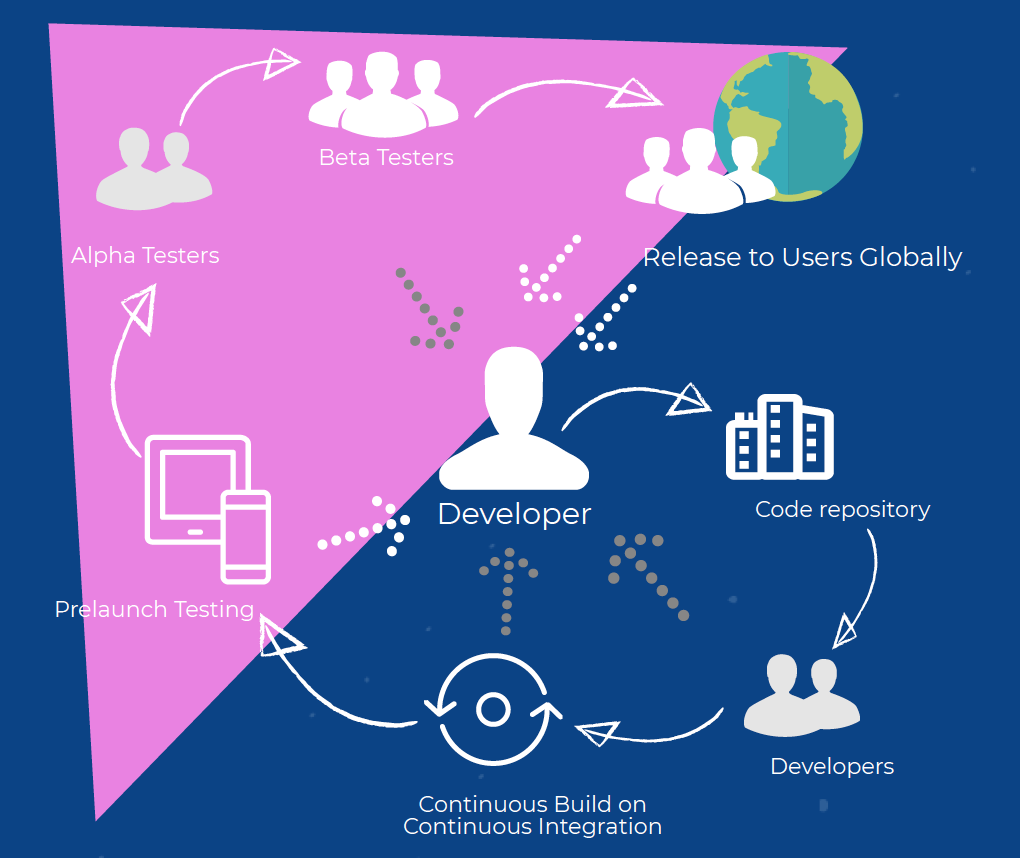
\includegraphics[width=14cm]{images/silvias-developer-centric-figure-mobilesoft2020.png}
    \caption[Sources of feedback for developers]{Sources of feedback for developers \\}
    \label{fig:sources-of-feedback-for-developers}
\end{figure}

\textbf{MUST-DO - fix this paragraph} Each source of feedback may stem from humans (for example, in reviews) or from software (for example, from code quality tools such as Lint).This research introduces three sources of software-generated feedback.


\section{Research Questions}
\label{section-research-questions}

My research hypothesis is that using mobile analytics can help improve both the work development teams do and the quality of the products they create. Here work includes the development, bug investigation, and testing of the software being created. For the quality of the product, this research is focusing on a subset of qualities which are technology-centric.

The domain of mobile apps was selected for this research as mobile apps are ubiquitous, extremely popular, and have interesting and challenging contexts of use. And, within the range of mobile apps, the research ended up focusing on Android apps for various reasons including: the analytics tools available, the relative glut of suitable apps available for research, my prior experience and expertise, and their market share.

The core question the research aims to consider is: 
\emph{How can applying analytics improve software development and software testing for mobile apps?}~\label{overall-research-question}
Here the assumption is that analytics can help, as stated by Buse and Zimmermann ~(\citeyear{buse_analytics_2010}); and \emph{``with explicit and implicit feedback now available (almost) continuously, questions arise. How can practitioners use this information and integrate it into their development processes [to decide when to release updates]?"}~\citep{maalej2016_towards_data_driven_requirements_engineering}.

This leads to several related questions that underpin this main question. These are grouped in three categories: sources, value, and impact.

%\akb{There are a lot of sub-questions below. You will need to focus on the ones you have data to evaluate, or have more abstract formulations that cover groups of sub-questions.}

\yijun{If possible, you may need to dig out a few MobileSoft research papers to give evidence that these research questions have not been addressed in literature, e.g., \emph{Future Trends in Software Engineering Research for Mobile Apps}~\citep{nagappan2016_future_trends_in_sw_eng_for_mobile_apps}, whether the future work of some paper suggests one does not know the sources, value, or impact of mobile analytics to assess and improve app quality? Is there nothing in the general SE literature studying the "analytics" to "general software quality" problem? If there are such general work, how does "mobile analytics" and "app quality" differentiate the RQs to existing ones...}



\subsection{Sources}~\label{section-sources}
At a superficial level, there seem to be mobile analytics offerings that operate within the app and those that are external to the app, particularly those that gather data at the platform level. Several widespread analytics offerings are evaluated as part of this research. Several more were considered to provide an understanding of the overall context.
\begin{itemize}
    \item \emph{What sources of analytics are available? And how do the sources that were investigated compare in terms of the data they collect and how they are used?}
    \item \emph{Hypothesis}: The various sources have distinct characteristics and purposes. Developers may wish to choose particular analytics to best suit their context and objectives.
\end{itemize}

\subsection{Value}~\label{section-value}
Does using analytics provide quantitative and/or qualitative value that can be measured? Could it provide value in terms of assessing the quality of our work that was invested into developing, testing and preparing software before it was launched?
\begin{itemize}
    \item \emph{How much does the fidelity of the analytics offerings matter?} Can the results be used productively even if they are flawed? The research discovered numerous errors in various analytics offerings. These results may be of interest to the research community given the endemic nature of mobile analytics in real-world apps in the major app stores.

    \item \emph{How can analytics help with bug investigation?} A single bug instance may be hard to assess in terms of the likely scope and impact on a user-base; how, where and when can analytics help with bug investigation? We might also consider practical limits,~\emph{e.g.,} constraints that are enforced by the real-world analytics we used. 
\end{itemize}

\subsection{Impact}~\label{section-impact}
Here the focus is on whether the value has sufficient impact for anyone else to be interested in using and applying analytics. Given the nature of the research the main measures are practical, \emph{i.e.}, in the real-world.
\begin{itemize}
    \item \emph{Do development teams use analytics in their practice?} If development teams find practices useful they will generally try to use them intrinsically. Do they? And if so, how?

\end{itemize}


\section{Potential sources of evidence}

%\emph{What can we learn from people? what can we learn from analytics? ...?}

%\textbf{How can we know about mobile analytics and the effects of using them?} 

%\nth{16} Jul 2021:~\akb{This subsection is too verbose. Summarise with a diagram showing sources of knowledge and links to difference types} - \textbf{MUST-DO} and will do once I make sense of where's the best place to put this material. For now I've moved the overall \href{section-ontology-and-episetemology}{\nameref{section-ontology-and-episetemology}} section to after the RQs and before the methodology section.

%Here we consider the questions: (1a) What we can know about mobile analytics and (1b) how we can know it? Then more specifically, these related questions are key given this research focuses on using mobile analytics to help answer the next question. (2) How we know about the identification and measurement of some flaws in behaviour of software that are considered measures of quality of the software in use? 

Broadly we can learn from people, use \textbf{software tools}~\footnote{\textbf{MUST-DO} This needs a paragraph}, and use data to answer these questions. In some cases the data comes from a single source, in others cases from several.



\textbf{Mobile analytics} comprises software, systems, and sometimes services. Broadly we can read about them, study their source code, analyse, test, and use them directly, and ask others for their perspectives and insights. Rather than go into lots of detail here, several of the appendices of this thesis cover aspects of mobile analytics, in particular, in~\href{app:on-mobile-analytics}{\emph{\nameref{app:on-mobile-analytics}}}. 

In terms of learning from \textbf{people}, we can do so by asking the designers, constructors, operators, and users of a system. However, we're also limited by who we can ask, what they are willing/able to communicate, and whether that communication is sufficiently open and transparent to be useful and reliable. We can also learn from information produced by people, and in particular for mobile apps we can use ratings and reviews. Given human behaviour it may also be worth considering aspects such as the provenance of the information sources, fake data, \emph{etc.} especially where there are rewards for slewing the results of the measurements being used in an ecosystem. 

We can know through \textbf{static analysis} tools, automated tests, end-to-end testing, \emph{etc.} and all of these are used by at least some of the developers of mobile apps some of the time. They often take place \textit{before} the software is released to end users.

We can also know through data collected when the software is used. As~\cite{RFC3164} notes in RFC3164, ~\emph{``Since the beginning... operating systems, processes and applications were written to send messages of their own status, or messages to indicate that certain events had occurred. These event messages generally had local significance to the machine operators."}. Mobile apps also write messages locally and developers use them for similar purposes (nuances and differences are discussed in the related work chapter). These local messages can be read by humans locally and/or read by software that delivers them elsewhere. Developers can also add software to their apps to log information for processing elsewhere which is where much of mobile analytics and crash reporting fits in the scheme of things.

Log messages are written locally on the same device (\textit{i.e.} computer) that runs the software. When developers are developing the software they tend to be local to the device and therefore able to read the logs. When the devices are remote, as they are for end users of mobile apps, developers cannot easily access the logs or read them. If they wish to do so they need mechanisms to obtain the logs. They can choose to incorporate mechanisms into the app including custom logging mechanisms that transmit the logs so they can be processed remotely. They can rely on log forwarding software~\footnote{For instance a fairly involved example for Flutter Android apps, using MQTT, is described in~\citep{adil2020_sending_logs_from_flutter_apps}}, and/or mechanisms provided on the device if they exist. 
% A couple of Android implementations for LogStash include:
%  https://github.com/Labgoo/android-logstash-logger
%  https://gist.github.com/PatrykGala/55603fe4259d812fdc0ffbc9e63eaabc (saved in my references)


Various data can be potentially collected implicitly and explicitly. What can be collected depends on the observation mechanisms. Observation may be within an app or external to it, for instance by the operating system as both iOS  and Google Android do~\footnote{There are other custom versions of Android, for instance used in Amazon Kindle Fire devices. Their details are outside the scope of my research.}(details in the Appendix titled~\href{chapter-on-mobile-analytics}{\emph{\nameref{app:on-mobile-analytics}}}). Within an app the observation may focus at a single layer, for instance the visual user interface, or several. The choices of observation mechanisms within an app are made by developers or their stakeholders. The choices external to an app can be made by various people including the platform provider, users, or indirectly using other software including third-party apps, spyware, accessibility software, and so on.

Analytics, such as user-journeys, can help to answer questions about the usage of the software. They help establish \emph{what-is}. As we understand more about what-is we can then consider \emph{what-would-be-better} and do gap analysis between what-is and what-would-be-better.

%See https://tex.stackexchange.com/questions/348298/svg-package-includesvg-with-underscores-in-svg
\makeatletter
\DeclareRobustCommand*{\escapeus}[1]{%
    \begingroup\@activeus\scantokens{#1\endinput}\endgroup}
\begingroup\lccode`\~=`\_\relax
    \lowercase{\endgroup\def\@activeus{\catcode`\_=\active \let~\_}}
\makeatother

%See https://tex.stackexchange.com/questions/390804/how-to-scale-text-in-svg
% PS: I could try https://tex.stackexchange.com/questions/113282/text-size-in-inkscape if I run into problems with the current approach.
\begin{figure}
\centering
    \copyrightbox[r]{
        \escapeus{\includesvg[pretex=\tiny,scale = 0.7]{images/github/loggerstructure.svg}}}
    {\textcopyright \href{{https://twitter.com/daroczig}}{daroczig}\\source: \href{https://github.com/daroczig/logger/blob/master/vignettes/logger\_structure.svg}{logger\_structure.svg}}
    \caption{TEMP - to be replaced: Logger Structure from an R Logger project - TBC whether to provide something similar}
    \label{fig:temp_logger_structure}
\end{figure}

\begin{comment}
%This is a simpler structure without the copyright box. Commented out for now, kept in case I want to switch quickly.
\begin{figure}[htbp!]
    \centering
    \escapeus{\includesvg[scale=1.0]{images/github/loggerstructure.svg}}
    \caption{Yin Yang to represent DevOps}
    \label{fig:yinyang_for_devopsxxx}
\end{figure}
\end{comment}


\textbf{Reporting/generating and Observing}: What happens within the app stays within the app unless someone looks inside the app or the app reports what's occurring. Observation without action limits the utility of whatever is learned.  \textbf{SHOULD-DO}, it'd be great to have a figure similar to \url{https://github.com/daroczig/logger/blob/master/vignettes/logger_structure.svg} for platform-level analytics. Temporarily it's included here in Figure~\ref{fig:temp_logger_structure}.


Survivorship bias (\cite{wikipedia_survivorship_bias}) is relevant to understanding the information developers receive, some data does not `survive' the journey from source to developer. And much of the information that is does reach the developers does not survive or, perhaps better put, thrive in terms of being used productively. They have plenty of other demands for their time and attention and much of what could be useful isn't used in practice, therefore the data needs to be sufficiently useful and relevant and improvements tractable for any proposed approach to be used long term in practice.


Discuss which sources are likely to provide input to the key elements needed to underpin the RQs.

\textbf{MUST-DO} Segue to the research strategy and how we devise a feasible approach that uses as many of these sources as practical.


\section{Research Strategy}
The research aims to provide practical and applicable insights to mobile apps developers. As such, the strategy was to work predominantly with development teams for mobile apps to ensure -- as far as practical -- that the research is externally validated through their experiences, practices and feedback. As developers need to make choices appropriate to their context, the research includes a variety of apps including commercial and not-for-profit, small, medium and large development teams and user bases, and has an international flavour with developers situated on various continents including Asia, Europe, and the USA.




\begin{comment}
    \begin{itemize}
        \item Get the audience to identify with someone or something, - Give that someone or something some kind of need, - And start changing the circumstances.
        \item Have that someone or something deal with the new circumstances - And find the thing that was needed.
        \item Have that someone or something pay the price of the find - And start heading back toward the original circumstances.
        \item show how those original circumstances have changed as a result.
    \end{itemize}
    \emph{Dan Harmon's story telling circle}
\end{comment}


\subsection{Case Studies}
Case studies have been established by various researchers as an effective method to understand software qualities, for instance in~\citep{khalid2014_prioritizing_the_devices_to_test_your_app_on_casestudy_android_games, khalid2015_what_do_mobile_app_users_complain_about, khalid2016_examining_the_relationship_between_findbugs_warnings_and_app_ratings, martinez_fernandez2019_continuously_assessing_and_improving_software_quality_with_software_analytics_tools}. And case studies are well suited to exploratory research, for which they may offer insights not available with other approaches~\citep{rowley2002_using_case_studies_in_research}, especially when events are contemporary and where the investigator has little or no control Chapter 1 in~\citep{yin2018_case_study_research_and_applications_6th_edition}. They are also recommended where the research includes multiple data sources~\citep{rowley2002_using_case_studies_in_research}. This research therefore uses case studies, as the research investigates real-world use of mobile analytics where many factors are outside the control of the researcher.

%In the research, developers were able to improve the measured reliability for each of the case studies despite flaws and limitations in the mobile analytics. Some improvements were gained with small amounts of effort; others were achieved through more strategic changes, including replacing Java code with Kotlin replacements and retiring buggy modules and external libraries.  

%Add a high level diagram or table of the case studies and what they provide.

\subsection{Analytics}

As my main research question considers the application of analytics, the research needs to include a combination of usage and analytics data, where the analytics data is then applied with the intent of improving the product quality. The developers may not be successful in achieving improvements, although we hope they will be. They may also be able to improve their practices, so again their current and revised processes are also of interest.

[Almost] anything can be measured sufficiently to be useful. In his book~\emph{How to Measure Anything, \nth{3} edition}~\citet{hubbard2014measure} argues that anything can be measured and proposes an approach to do so. His framework, called \emph{Applied Information Economics: A Universal Approach to Measurement}, is summarised in five steps:

\begin{enumerate}
    \item Define the decision.
    \item Determine what you know now.
    \item Compute the value of additional information. (If none, go to step 5.)
    \item Measure where the information value is high. (Return to steps 2 and 3 until further measurement is not needed.)
    \item Make a decision and act on it. (Return to step 1 and repeat as each action creates new decisions.)
\end{enumerate} ~\cite[p.9]{hubbard2014measure}.

This approach helps to frame this research into applying analytics to development practices, especially in terms of the practical aspects and nature of real-world apps, development teams, and user-bases.




\subsection{Perspectives of the developers of the apps and the tools}
As the analytics tools also influence the results, the research includes discussions and collaborations with several organisations who create these tools.

This research is not immune from also being improved, and similarly the process is likely to have plenty of scope for improvement as we learn more from the various projects, teams, apps, and analytics tools. Similarly, there is scope to find flaws, limitations, and weaknesses in the analytics tools; therefore there was scope in the research to share findings with the teams responsible for these, and related, software tools and to use the experiences and insights from any such sharing as part of this research.



\subsection{Triangulation}
Where practical, triangulation~\footnote{c.f. collegation} of data and analytics reports was used to help increase the confidence in the analytics and in the efficacy of using mobile analytics. As~\citep{marr2015bigdatabook} recommends:~\emph{``Measure metrics and data backed up or triangulated with other data sources."} and~\emph{``Where possible use a combination of data sets and triangulate the data. In other words, see if each data set delivers the same result so you can confirm and validate the answers."}. Triangulation of research methods is extensively covered in research. For example, \citep{fielding2012_triangulation_and_mixed_methods_designs} provides a rich discussion of triangulation and mixed methods design for various research areas. To the best of my knowledge  %SHOULD-DO decide how much to focus on triangulation, whether to discuss data triangulation as a technique for comparing analytics results (which doesn't seem to quite apply - at least in what I've read).

The next level of validity was that even if this work achieved the desired results, could other development teams achieve similar results by applying a similar approach? To help gain evidence, the research engaged a separate opensource development project and development team. 

Cross validation through multiple case studies. Comparing opensource and commercial projects for their approaches and results. Multiple ecosystems. Data types and informant types. Choice of case studies intended to provide variety and the opportunity for comparison. Multi-layered approach.

%\section{My research methodology, and my choices}
Needs full rework.

Merge into the strategy
Headings: 
- case study approach
- data collection
- (remove 'action research' from the introduction as it's not the strategy, instead mention it in the relevant case study: Kiwix).

draft wording for a high-level scene setting: Within these case studies there were particular needs that led to choices in the specific case studies: 


May RQ's to the case studies and explain how they're mapped, and the methods I'll be introducing later on. High level choices of the key choices I made in order to answer the RQs. Map in Chapter 3.



%Move to the case study that used the action research: 
%Although I had prior experience in industry of the efficacy and potency of applying usage analytics to improve software development and testing of mobile apps, that experience was generally covered by confidentially agreements, and also the analytics tools have changed and developed markedly since those experiences. Therefore, action research seemed appropriate, particularly as one of the long-term opensource projects had extremely high failure rates according to the \emph{de facto} Android analytics tool. I decided it was appropriate and necessary to see if I could help that project directly to improve their mobile apps -- \emph{``physician heal thyself"}\footnote{\href{https://en.wikipedia.org/wiki/Physician,\_heal\_thyself}{wikipedia.org/wiki/Physician,\_heal\_thyself}.}.









\begin{comment}
    - Could I try phrasing my RQs as OKRs to see if doing so helps me to improve the clarity and relevance of the RQs.
    - Also, how about creating annotated editions of my RQs where the annotations include context, commentary, connections to other RQs, notes on twitter-style answers to each, etc.
    - We want to know more about 'this' topic. Then provide Operational questions - to be addressed by the research, which will help us learn more about the topic.
    - What's a RQ and what's an analytical lens (to be used to help with the RQ)?
\end{comment}




\begin{comment}
    

\section{Ontology and Epistemology}~\label{section-ontology-and-episetemology}
This section introduces the theoretical perspective in terms of the ontology and epistemology in terms of using mobile analytics for improving app quality.~\footnote{
\begin{itemize}
    \item Ontology \( \rightarrow \) a theory of `being' (existence).
    \item Epistemology \( \rightarrow \) what we can know about the microcosm/the world and how we can know it (a theory of knowledge).
\end{itemize}

Both these definitions are taken from~\cite{marsh2002skin}. While the article is aimed at social science research, it introduces both topics and their relationships clearly and practically~\footnote{Note: newer versions of the introductory material is published in a book: \href{https://www.macmillanihe.com/page/detail/Theory-and-Methods-in-Political-Science/?K=9781137603517}{\emph{``Theory and Methods in Political Science (\nth{4} Edition)".}}}.
}

\end{comment}

%Could also be used as a lens for applying analytics.




\section{Outline of this thesis}
% This is a placeholder, to be reviewed and updated when the thesis is closer to completion.
\begin{enumerate}
    \item This research is informed by and situated in the context of that of many others;
    \item 
    \item 
    \item 
    \item 
    \item 
    \item 
    \item     
\end{enumerate}
 Chapter 2 sets this research into the wider research context. 
Chapter 3 prepares the ground by providing various concepts and the practical context for the research. 
The case studies performed as part of this research are in the \nth{4} chapter, followed by the key software developed to facilitate, support, and enable some of the case studies in Chapter 5.
Chapter 6 sums up the findings and results; then Chapter 7 evaluates the research.
Chapter 8 draws on what was learned and discovered in the case studies to help future researchers and practitioners find ways to apply usage analytics to development practices.
Chapter 9 discusses the research in a wider context beyond the immediate case studies.
Chapter 10 concludes this research, and Chapter 11 considers future, further work.
After the bibliography there are various appendices for those interested. 



%%%%%%%%%%%%%%%%%%%%%%%%%%%%%%%%%%
\par\noindent\rule{\textwidth}{0.4pt}
%%%%%%%%%%%%%%%%%%%%%%%%%%%%%%%%%%


